\documentclass[11pt]{beamer}

\usetheme{metropolis}

\usepackage{graphicx}
\usepackage{physics}
\usepackage{adjustbox}
\usepackage{caption}
\usepackage{chemformula}
\usepackage{quoting}
\usepackage[style=chem-angew,backend=bibtex]{biblatex}
\bibliography{references}
%
% Choose how your presentation looks.
%
% For more themes, color themes and font themes, see:
% http://deic.uab.es/~iblanes/beamer_gallery/index_by_theme.html
%
\mode<presentation>
{
  \usetheme{default}      % or try Darmstadt, Madrid, Warsaw, ...
  \usecolortheme{default} % or try albatross, beaver, crane, ...
  \usefonttheme{default}  % or try serif, structurebold, ...
  \setbeamertemplate{navigation symbols}{}
  \setbeamertemplate{caption}[numbered]
  \setbeamerfont{footnote}{size=\tiny}
} 

\usepackage[english]{babel}
\usepackage[utf8]{inputenc}
\graphicspath{{image/}}

\AtBeginSection[]{
\begin{frame}{Outline}
  \tableofcontents[currentsection]
\end{frame}
}

\title{Chapter 10+11: Intermolecular Forces}
\institute{Chemistry Department, Cypress College}
\date{Dec 5, 2022}

\begin{document}

\begin{frame}
  \titlepage
\end{frame}

\begin{frame}{Class Announcements}
  \textbf{Lecture}
  \begin{itemize}
  \item Short lecture Ch 10 and 11
  \item Final Exam Dec 10th in Lecture
  \item Turn in all assignments
  \end{itemize}
\end{frame}

\section{Review: Dalton's Law of Partial Pressures}

\begin{frame}{Dalton's Law of Partial Pressures}
  Gases in a mixture behave independently and exert the same pressure they would
  exert if they were in a container alone
  \begin{equation}
    P_\text{Total} = P_A + P_B + P_C + \cdots
  \end{equation}
  where $P_\text{Total}$ is the total pressure and $P_A, P_B, \cdots$ are the
  pressures of the components
\end{frame}

\begin{frame}{Dalton's Law of Partial Pressures}
  \begin{center}
    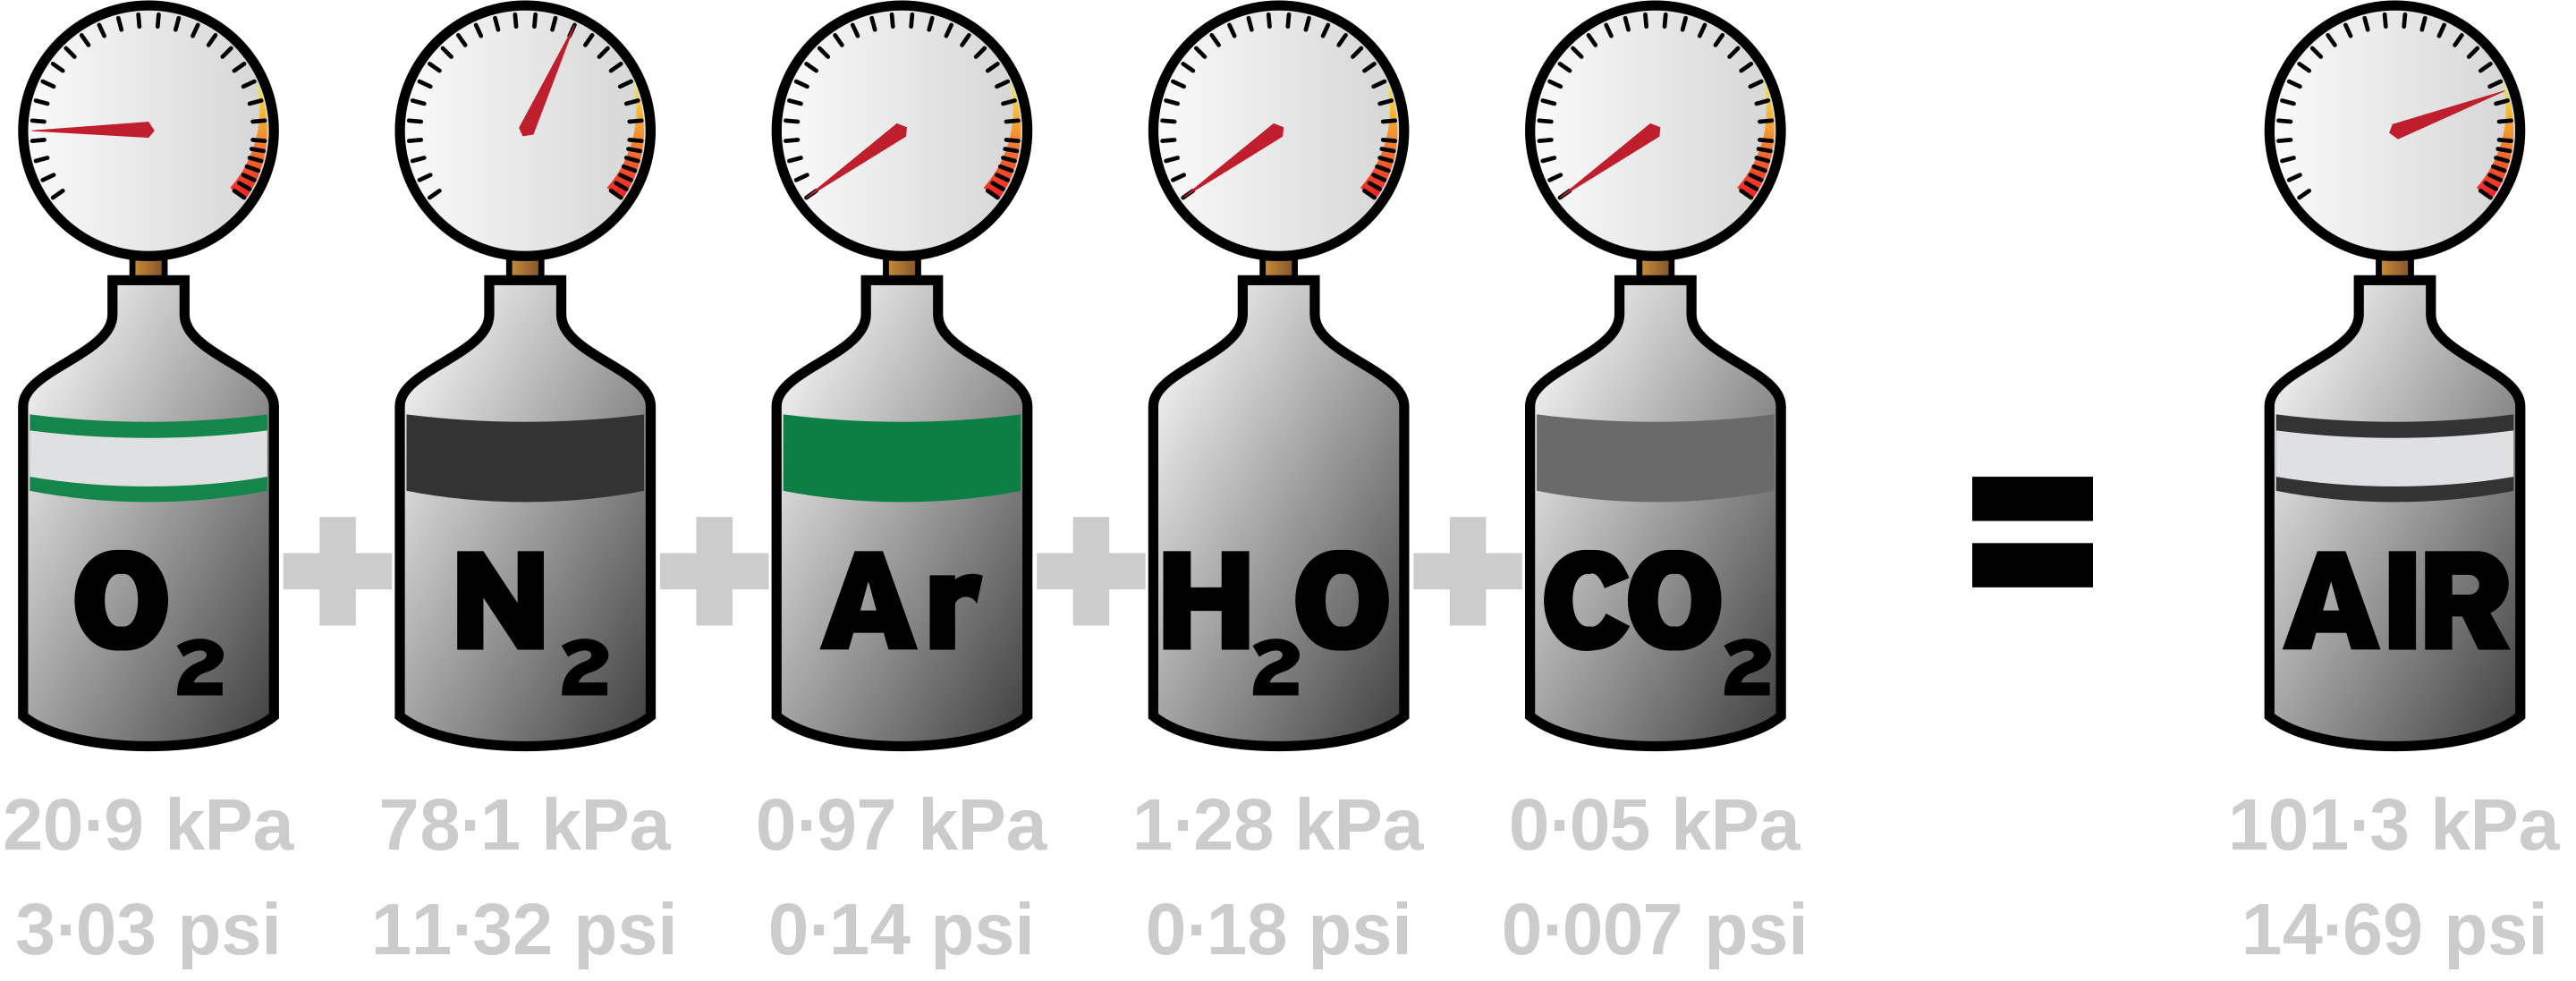
\includegraphics[width=\linewidth]{dalton_partial}
  \end{center}
  \begin{equation}
    P_\text{Total} = P_\text{O2} + P_\text{N2} + P_\text{Ar}
    + P_\text{H2O} + P_\text{CO2}
    \nonumber
  \end{equation}
\end{frame}

\begin{frame}{Mole Fraction}
  Expressing the relative amounts of substances in a mixture
  \begin{equation}
    \chi_A = \frac{n_A}{n_\text{Total}}
  \end{equation}
  where $\chi_A$ is the mole fraction of component A, $n_A$ is the
  amount of moles for A, and $n_\text{Total}$ is the total amount of
  moles in the mixture
\end{frame}

\begin{frame}{Dalton's Law of Partial Pressure}
  Since each gas component exert its own pressure, the partial pressure
  of each component can be expressed by
  \begin{equation}
    P_A = \chi_A P_\text{Total} = \frac{n_A}{n_\text{Total}} P_\text{Total}
  \end{equation}
\end{frame}

\section{Intermolecular Forces}

\begin{frame}{Introduction: Gecko's Sticky Secret}
  \center
  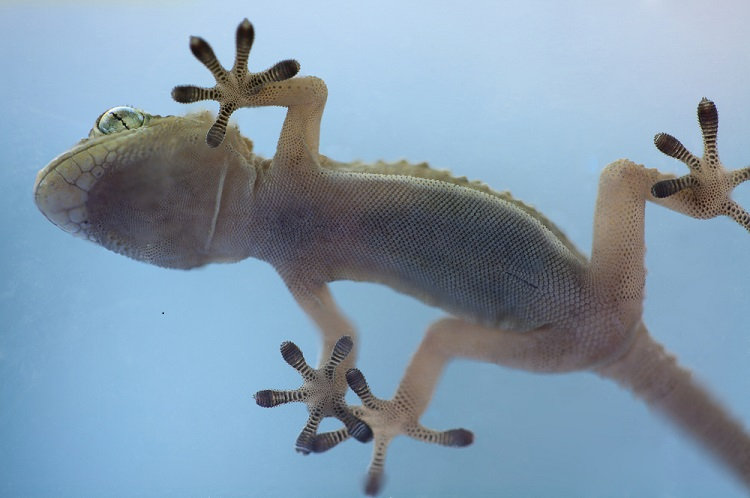
\includegraphics[width=0.475\textwidth]{gecko-feet.jpg}
  \hfill
  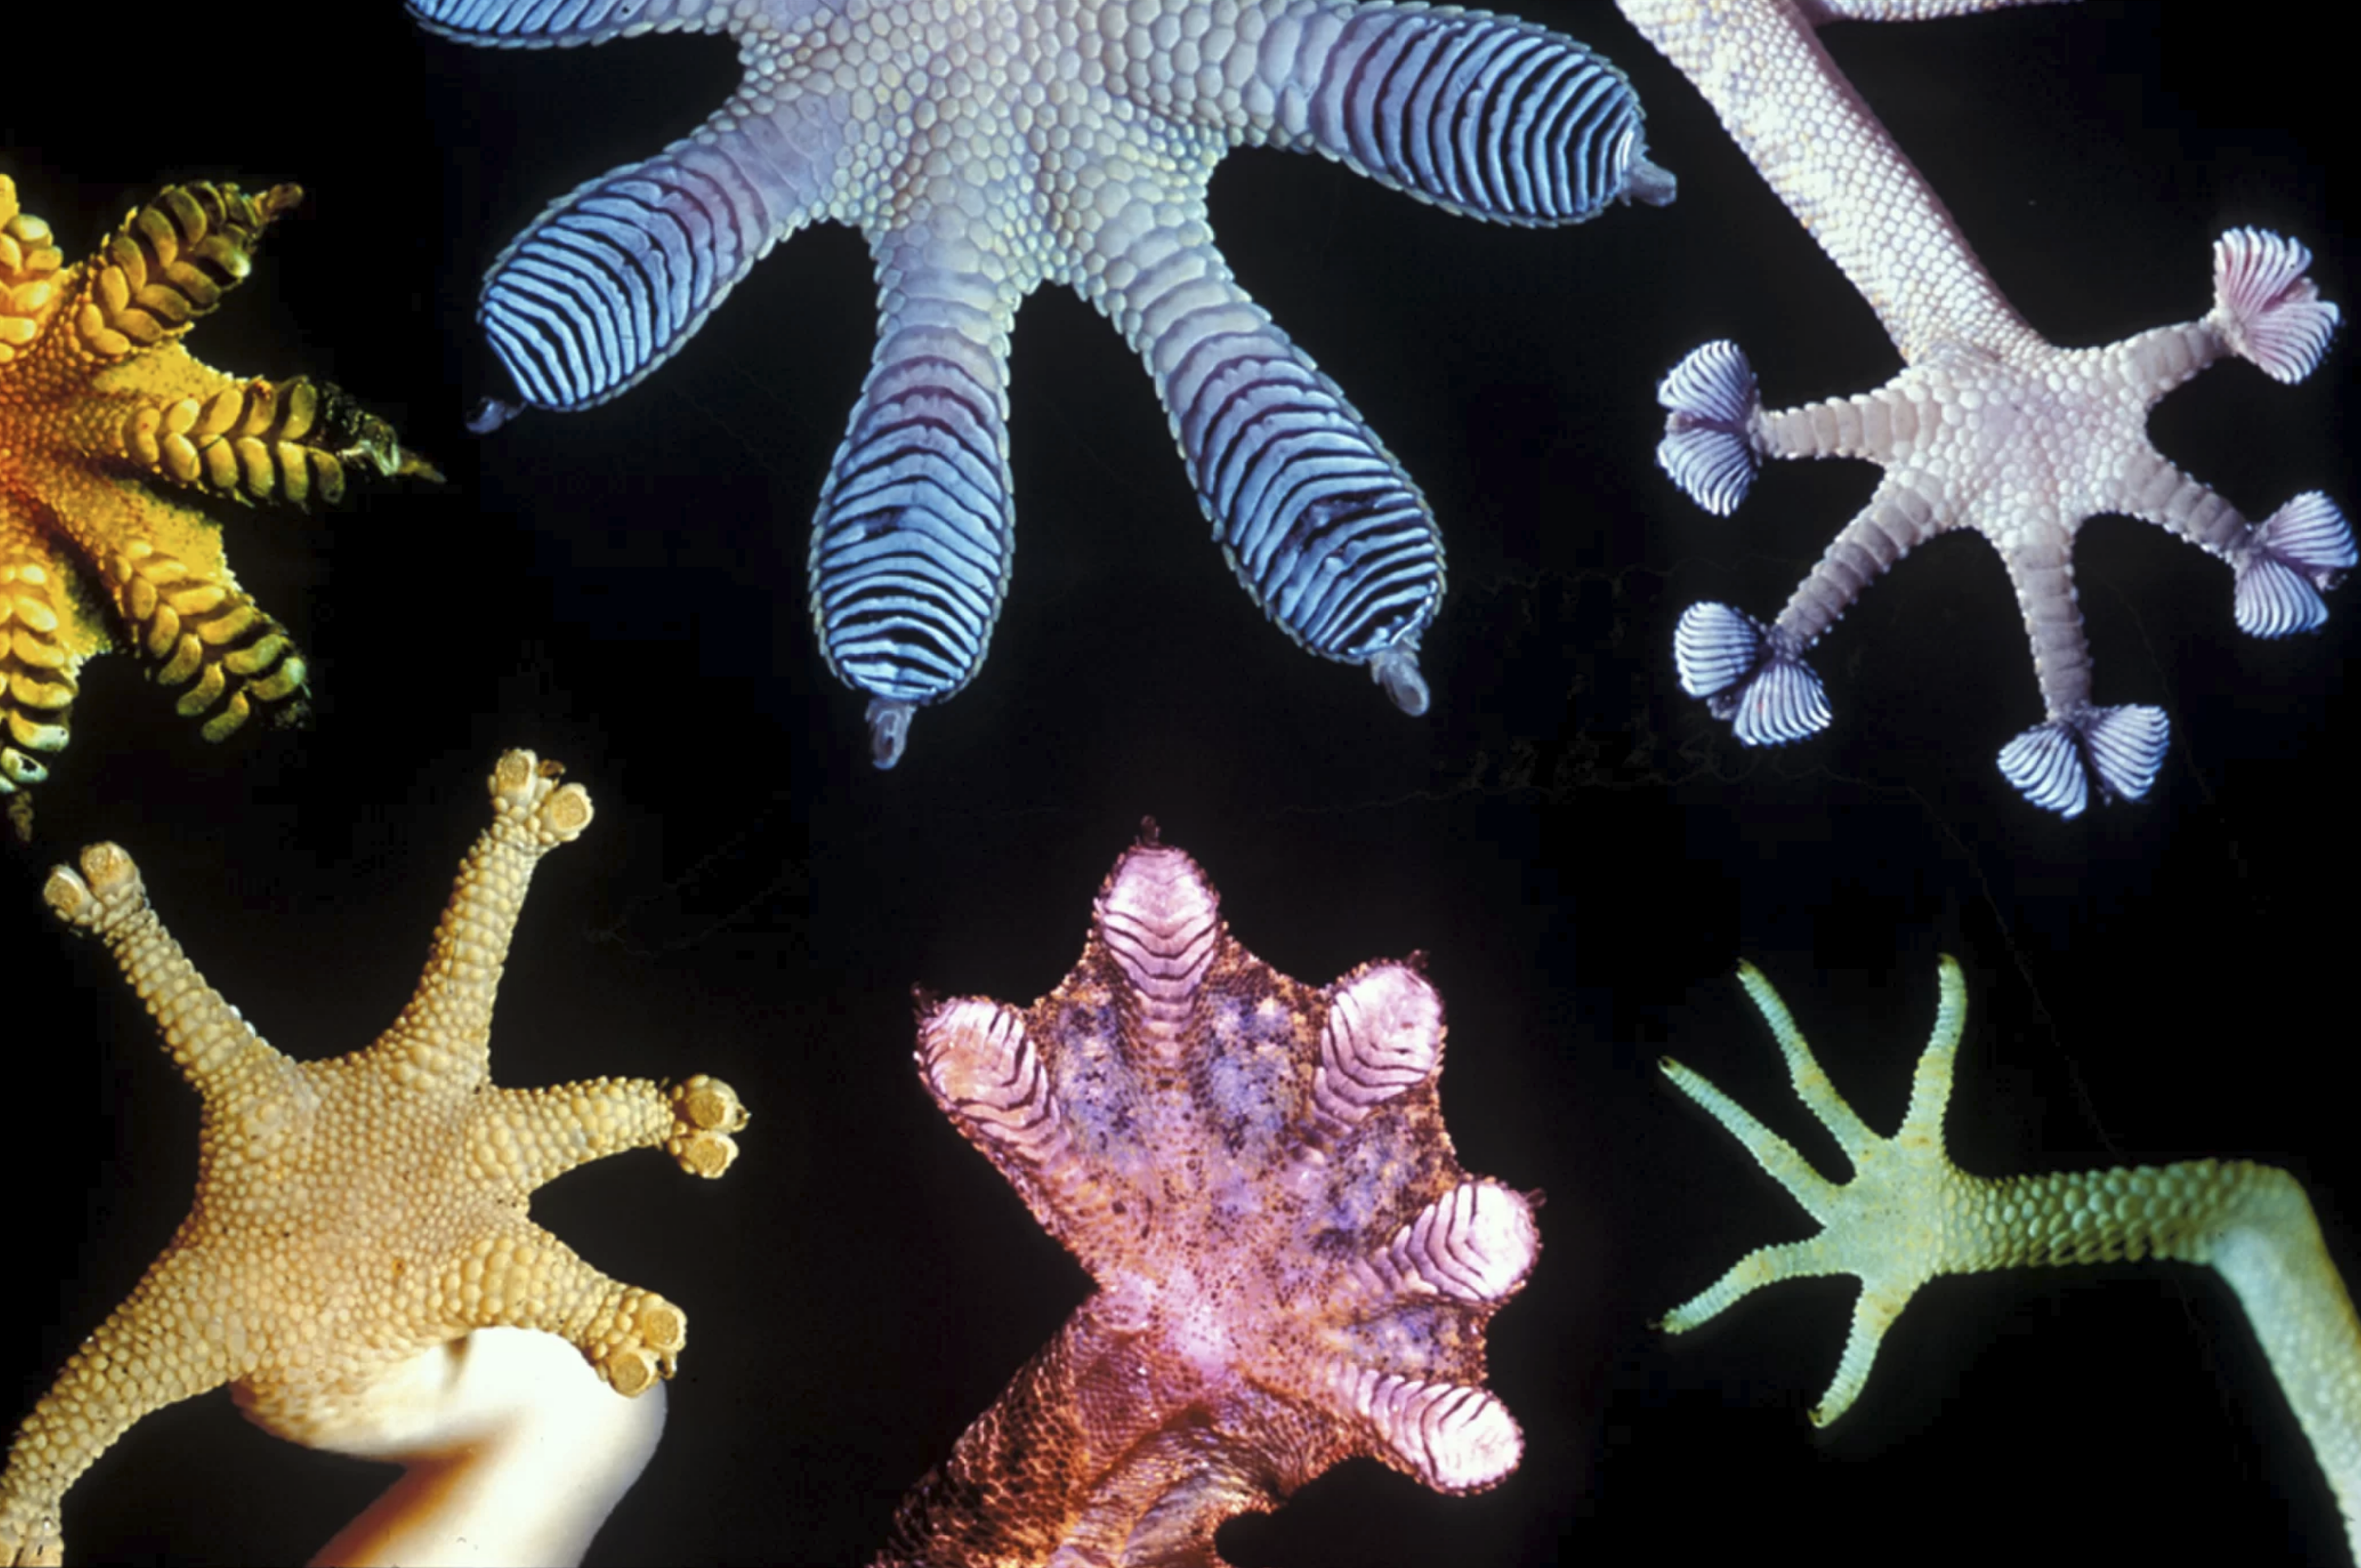
\includegraphics[width=0.475\textwidth]{inspired_feet.png}
  \begin{itemize}
    \item Quickly turn their feet on/off (literally hanging by
      their toe hairs)
    \item Dominated by intermolecular forces
    \item Gecko-inspired materials e.g. sealing wounds and scaling
      walls
  \end{itemize}
\end{frame}

\begin{frame}{Defining Intermolecular Forces}
  \textbf{Intermolecular forces} - interactions between molecules
  and significantly weaker than chemical bonds on the order of
  $\sim 10 - 10^3$ kJ/mol
\end{frame}

\begin{frame}{Types of Intermolecular Forces}
  \begin{center}
    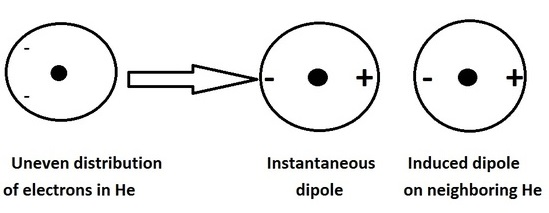
\includegraphics[scale=0.45]{disp.jpg}
  \end{center}
  \textbf{London Dispersion Forces} - Spontaneous induced dipoles
  and weakest intermolecular forces; the heavier the molecule then
  the stronger these interactions (molar mass dependence)
\end{frame}

\begin{frame}{Types of Intermolecular Forces}
  \begin{center}
    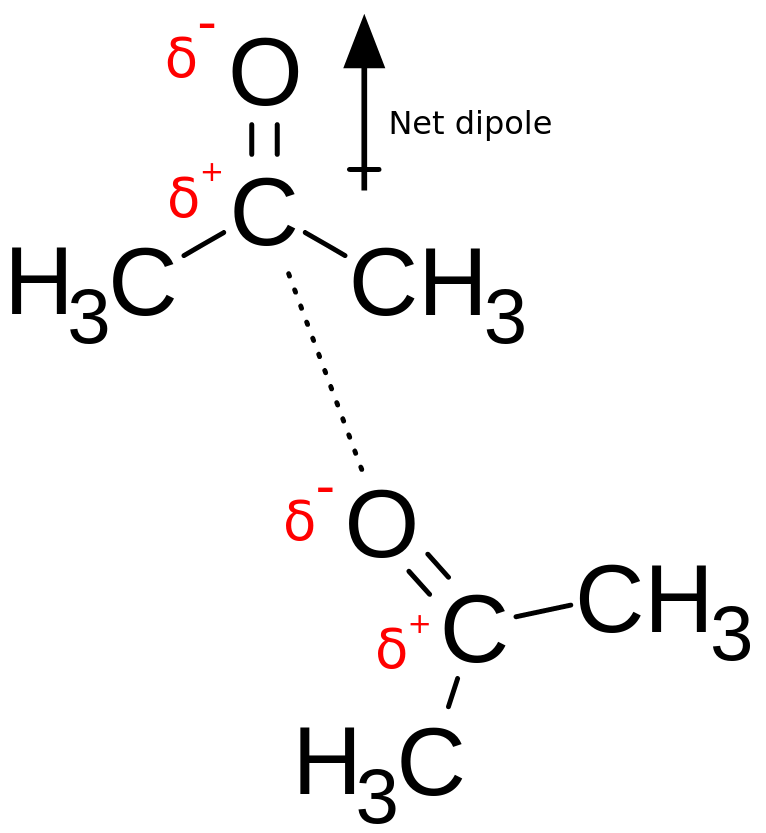
\includegraphics[width=0.4\linewidth]{dipole_dipole}
  \end{center}
  \textbf{Dipole-dipole interactions} - attractions between polar
  molecules; stronger than dispersion
\end{frame}

\begin{frame}{Types of Intermolecular Forces}
  \begin{center}
    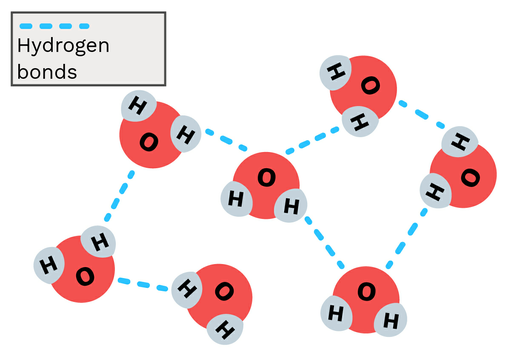
\includegraphics[width=0.5\linewidth]{water_hbond}
  \end{center}
  \textbf{Hydrogen bonds} - when H atoms are bonded to
  N, O, and F forming strong dipoles due to large electronegativity
  difference; strongest intermolecular forces
\end{frame}

\begin{frame}{Practice: Identify the Intermolecular Forces}
  Determine the intermolecular forces present in the following molecules:

  CO$_2$

  H$_2$O

  CH$_4$

  PF$_4$

  BH$_3$

  C$_{12}$H$_{26}$
\end{frame}

\begin{frame}{Practice: Identify the Intermolecular Forces}
  Based on the answers in the previous slide, rank the molecules
  from strongest to weakest intermolecular forces
  
  CO$_2$

  H$_2$O

  CH$_4$

  PF$_4$

  BH$_3$

  C$_{12}$H$_{26}$
\end{frame}

\begin{frame}{Practice: Identify the Intermolecular Forces}
  Based on the answers in the previous slide, rank the molecules
  from highest to lowest boiling point
  
  CO$_2$

  H$_2$O

  CH$_4$

  PF$_4$

  BH$_3$

  C$_{12}$H$_{26}$
\end{frame}

\begin{frame}{Relating Vapor Pressure}
  \begin{center}
    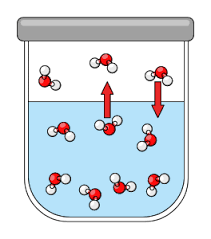
\includegraphics[width=0.3\linewidth]{vapor_pressure}
  \end{center}
  \begin{itemize}
  \item Equilibrium between gas and liquid phase of the molecule
  \item Vapor pressure correlates with the strength of the
    intermolecular forces present in molecules
  \item \textbf{Q}: Determine which has higher vapor pressure:
    NH$_3$ or CH$_2$O
  \end{itemize}
\end{frame}

\begin{frame}{Relating Vapor Pressure}
  \begin{center}
    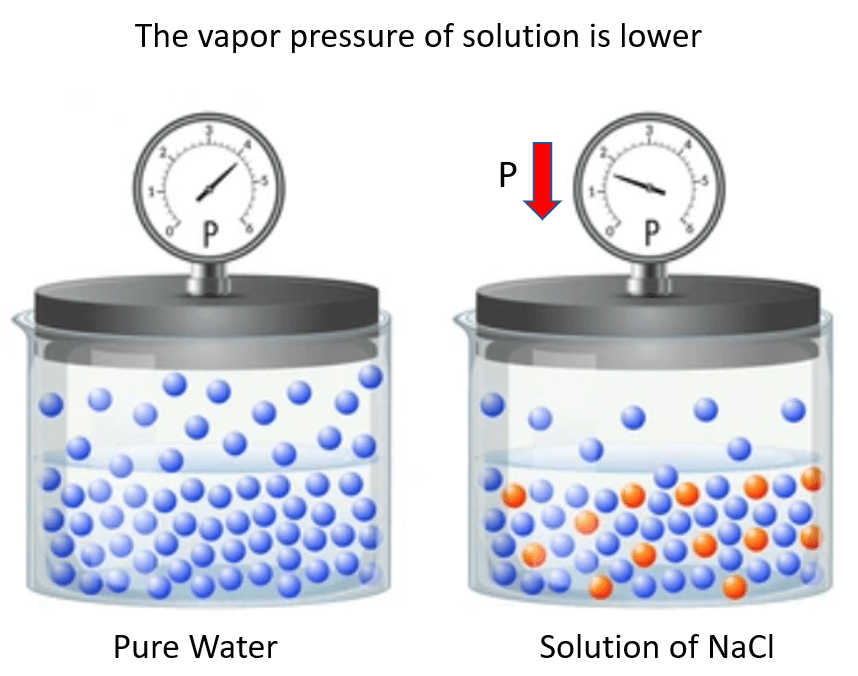
\includegraphics[width=0.7\linewidth]{soln_vp}
  \end{center}
  \textbf{Q}: How does the presence of NaCl lower the vapor
  pressure of water?
\end{frame}

\begin{frame}{Vapor Pressure and Boiling}
  \centering
  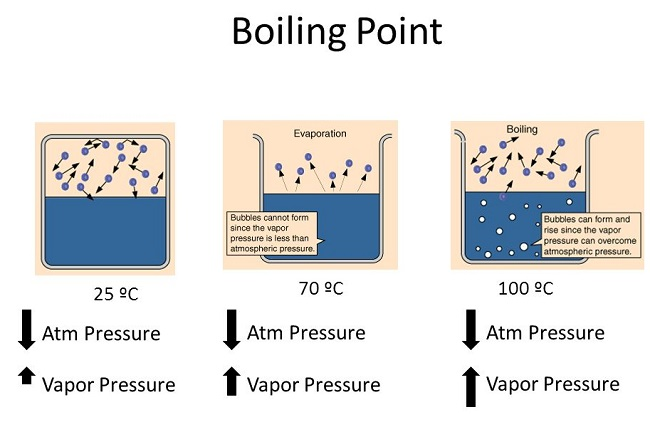
\includegraphics[width=\linewidth,trim={0 0 0 1in},clip]{boiling_vapor}
\end{frame}

\section{Heating Curves: Melting and Boiling Point}

\begin{frame}{Heating Curves}
  \centering
  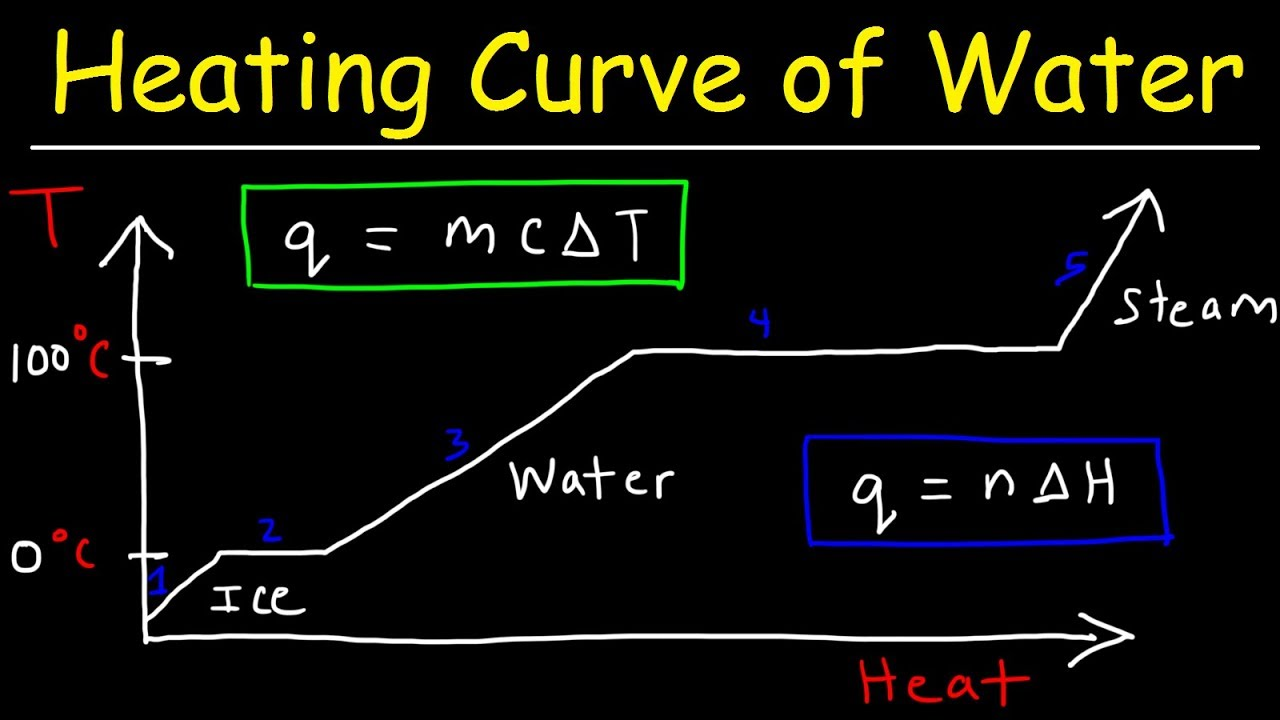
\includegraphics[width=\linewidth]{heating_curve_h2o}
\end{frame}

\begin{frame}{Practice: Heat Energy}
  Calculate the heat absorbed when 125g H$_2$O(s) at -10$^\circ$C
  is converted to H$_2$O(g) at 150$^\circ$C. The specific heats of ice,
  water, and water vapor are 2.03 J/(g $^\circ$C), 4.18 J/(g $^\circ$C),
  and 2.02 J/(g $^\circ$C), respectively. the molar heat of fusion of ice
  is 6,010 J/mol and heat of vaporization of water is $4.07 \times 10^4$
  J/mol.
  \vspace{1.4in}
\end{frame}

\section{Molarity: Precipitation and Acid-Base Reactions}

\begin{frame}{Balanced Chemical Equation: Photosynthesis}
  \centering
  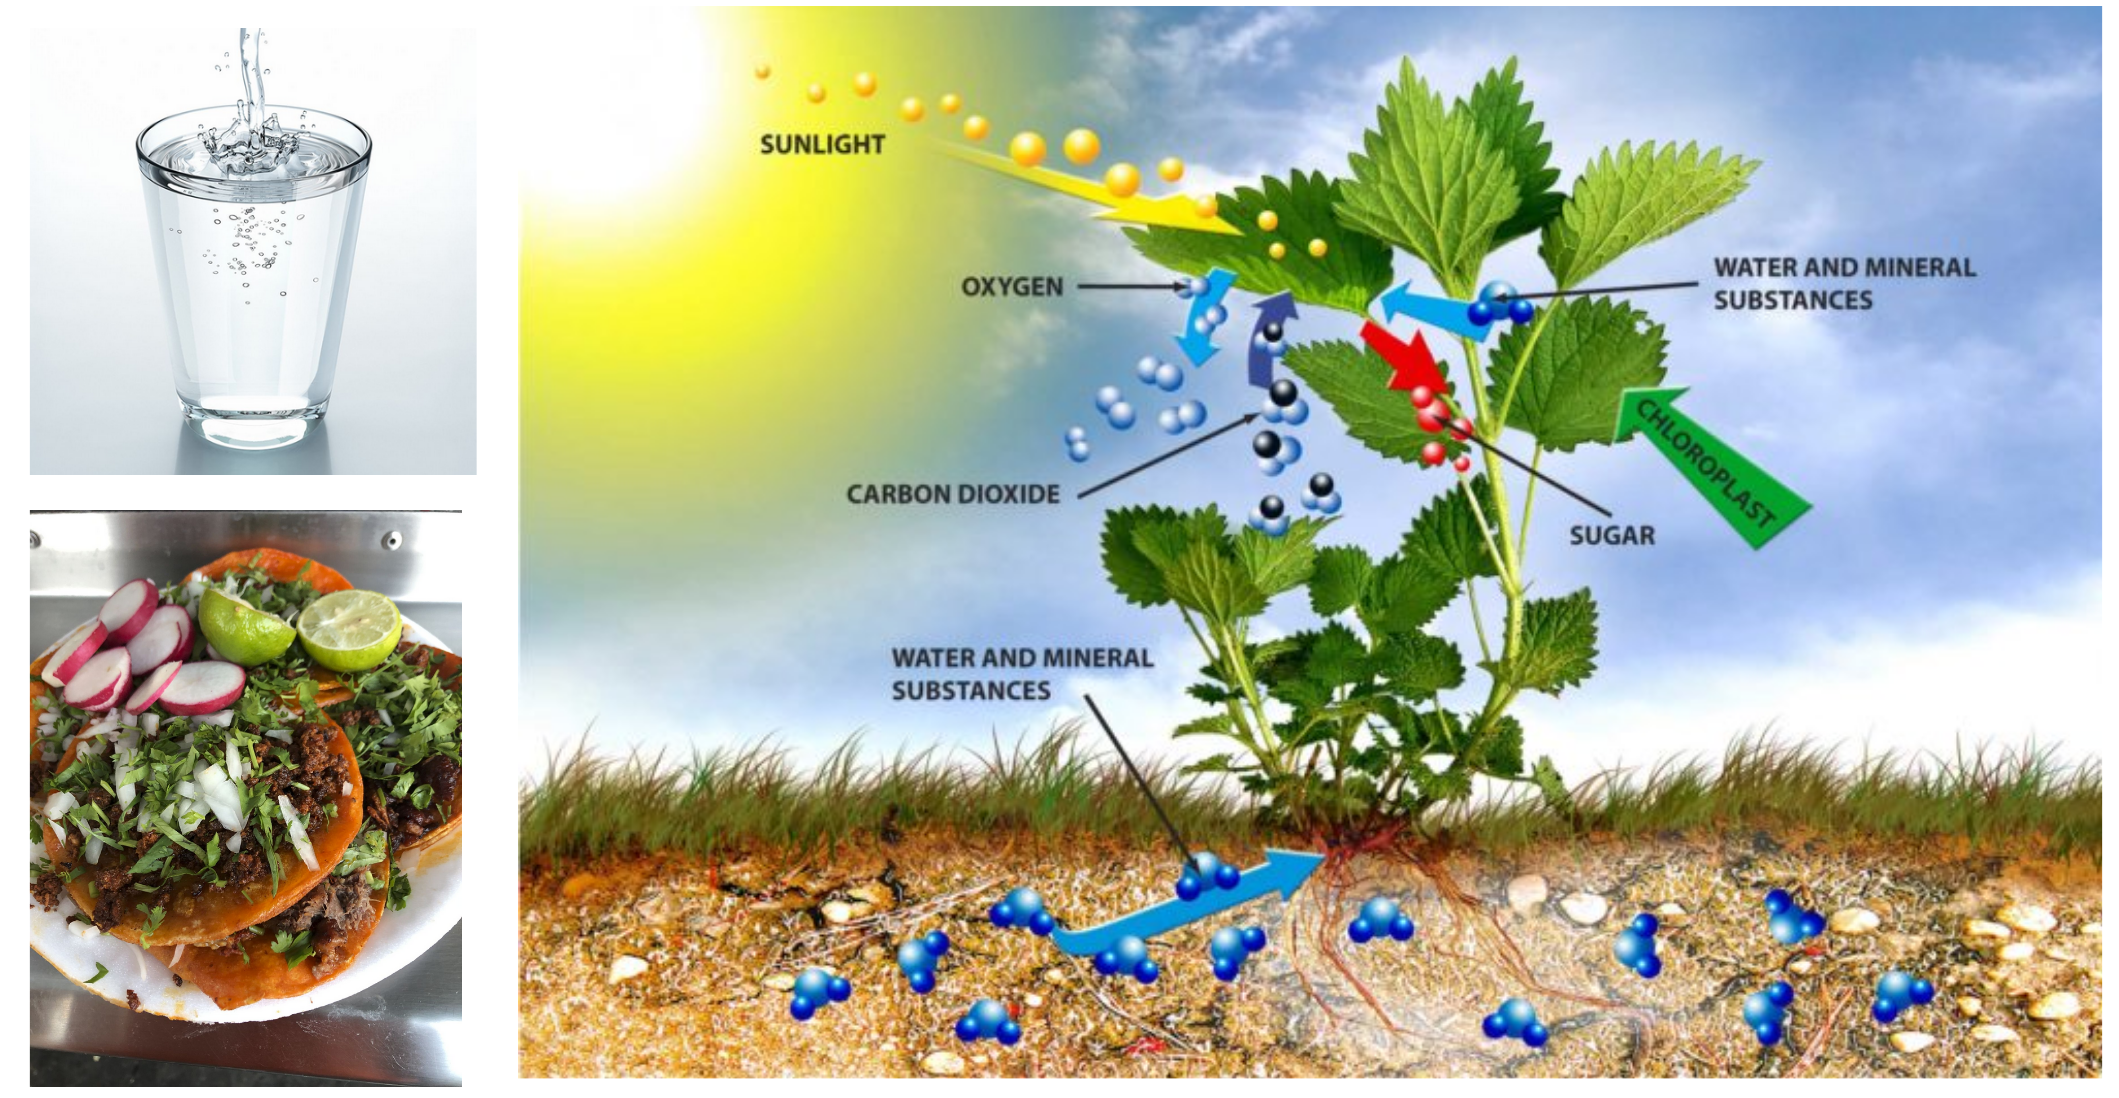
\includegraphics[trim={8in 0 0 0},clip,width=1\linewidth]{food_pic}
\end{frame}

\begin{frame}{Meaning of a Balanced Equation}
  \textbf{Photosysnthesis Chemical Equation}
  \begin{equation}
    6\text{CO$_2$(g)} + 6\text{H$_2$O(l)} \rightarrow \text{C$_6$H$_{12}$O$_6$(s)}
    + 6\text{O$_2$(g)}
  \end{equation}
  
  \begin{itemize}
  \item Balanced chemical equation satisfies the conservation of mass
  \item Coefficients in front of the molecules represent the relative
    moles of reactants and products
  \end{itemize}
\end{frame}

\begin{frame}{Practice: Precipitation Reaction}
  Suppose we want to prepare BaSO$_4$(s) by adding 0.450 M K$_2$SO$_4$(aq) to
  130.0mL of 0.250 M BaCl$_2$(aq). What volume of K$_2$SO$_4$(aq) is needed
  to react completely with the BaCl$_2$(aq)? How many grams of BaSO$_4$ will
  precipitate?
  \vspace{1.5in}
\end{frame}

\begin{frame}{Practice: Acid-Base Reaction}
  Suppose a titration is run in which 35.00mL of NaOH(aq) solution of unknown
  concentration reacts with 25.00mL of 0.100M H$_2$SO$_4$(aq). What is
  the molarity of the NaOH solution?
  \vspace{1.5in}
\end{frame}

\begin{frame}{Practice: Acid-Base Reaction}
  Suppose you neutralize 50.0mL of 2.5M H$_3$PO$_4$(aq) with 1.25M NaOH(aq).
  Determine the volume of 1.25M NaOH(aq) needed to neutralize H$_3$PO$_4$(aq)?
  \vspace{1.5in}
\end{frame}

\end{document}
